\chapter{Trees and Binary Trees}\label{ch09:trees-and-binary-trees}

\section{Introduction}

Trees are the most important non-linear data structure in computing. They organize data hierarchically — file systems, parse trees, decision trees, and search structures all use trees.

A \textbf{tree} consists of \textbf{nodes} connected by \textbf{edges}. Each node has exactly one \textbf{parent} (except the \textbf{root}, which has none) and zero or more \textbf{children}. Nodes with no children are \textbf{leaves}.

> \textbf{Complete compilable implementations of the data structures in this chapter are in \texttt{code/}.}

\section{Terminology}

\begin{figure}[ht]
\centering
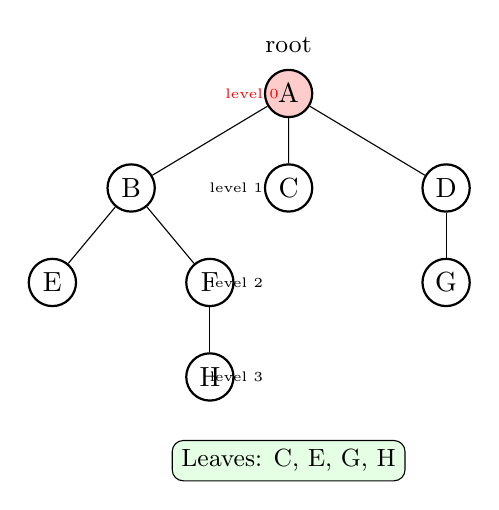
\begin{tikzpicture}
\tikzstyle{t}=[draw,circle,minimum size=0.6cm,inner sep=2pt,thick]
\node[t,fill=red!20] (A) at (2,0) {A};
\node[t] (B) at (0,-1.2) {B};
\node[t] (C) at (2,-1.2) {C};
\node[t] (D) at (4,-1.2) {D};
\node[t] (E) at (-1,-2.4) {E};
\node[t] (F) at (1,-2.4) {F};
\node[t] (G) at (4,-2.4) {G};
\node[t] (H) at (1,-3.6) {H};
\draw (A) -- (B) (A) -- (C) (A) -- (D);
\draw (B) -- (E) (B) -- (F);
\draw (D) -- (G);
\draw (F) -- (H);
\node[above] at (2,0.4) {\small root};
\node[left,red] at (2,0) {\tiny level 0};
\node[left] at (1.8,-1.2) {\tiny level 1};
\node[left] at (1.8,-2.4) {\tiny level 2};
\node[left] at (1.8,-3.6) {\tiny level 3};
\node[draw,rectangle,rounded corners,fill=green!10,below] at (2,-4.4) {\small Leaves: C, E, G, H};
\end{tikzpicture}
\end{figure}

\begin{itemize}
\item \textbf{Root:} A (no parent)
\item \textbf{Parent/Child:} A is parent of B, C, D; B is child of A
\item \textbf{Leaf:} C, E, G, H (nodes with no children)
\item \textbf{Siblings:} B, C, D share parent A
\item \textbf{Path:} sequence of connected nodes: A $\to $ B $\to $ F $\to $ H
\item \textbf{Path length:} number of edges on a path (3 for A to H)
\item \textbf{Depth of node:} path length from root (depth of H = 3)
\item \textbf{Height of node:} longest path from node to a leaf (height of B = 2)
\item \textbf{Height of tree:} height of root (height = 3)
\item \textbf{Subtree:} any node and its descendants
\item \textbf{Degree:} number of children (A has degree 3, H has degree 0)
\end{itemize}

\section{Binary Trees}

A \textbf{binary tree} is a tree where each node has at most 2 children: \textbf{left} and \textbf{right}.

\subsection{Properties}

\begin{enumerate}
\item Maximum nodes at level i: 2$^{i}$
\item Maximum nodes in a tree of height h: 2$^{h}$$^{+1}$ - 1
\item Minimum height of a tree with n nodes: $\lceil $log$_{2}$(n+1)$\rceil $ - 1
\item A \textbf{full binary tree} has every node with 0 or 2 children.
\item A \textbf{complete binary tree} is full except possibly the last level, which is filled left to right.
\item A \textbf{perfect binary tree} has all leaves at the same level.
\end{enumerate}

\textbf{Internal path length:} sum of depths of all internal (non-leaf) nodes.  
\textbf{External path length:} sum of depths of all leaves.

\begin{figure}[ht]
\centering
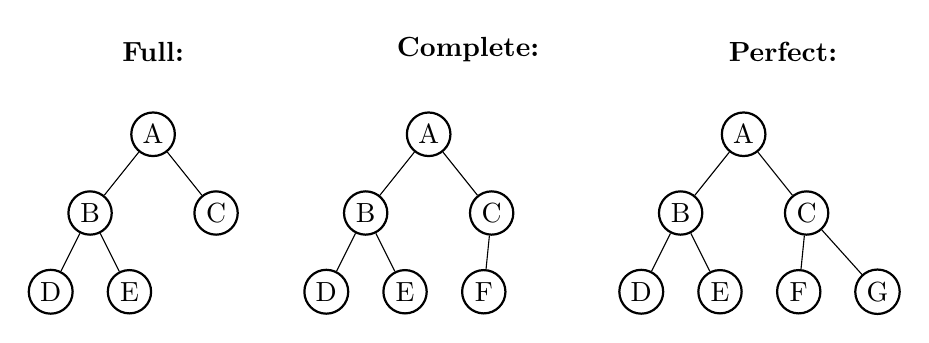
\begin{tikzpicture}
\tikzstyle{t}=[draw,circle,minimum size=0.55cm,inner sep=2pt,thick]
\tikzstyle{tn}=[t,fill=gray!15]

% Full binary tree
\node[above] at (0,0.3) {\textbf{Full:}};
\node[t] (a) at (0,-0.5) {A};
\node[t] (b) at (-0.8,-1.5) {B};
\node[t] (c) at (0.8,-1.5) {C};
\node[t] (d) at (-1.3,-2.5) {D};
\node[t] (e) at (-0.3,-2.5) {E};
\draw (a)--(b) (a)--(c) (b)--(d) (b)--(e);

% Complete binary tree
\node[above] at (4,0.3) {\textbf{Complete:}};
\node[t] (f) at (3.5,-0.5) {A};
\node[t] (g) at (2.7,-1.5) {B};
\node[t] (h) at (4.3,-1.5) {C};
\node[t] (i) at (2.2,-2.5) {D};
\node[t] (j) at (3.2,-2.5) {E};
\node[t] (k) at (4.2,-2.5) {F};
\draw (f)--(g) (f)--(h) (g)--(i) (g)--(j) (h)--(k);

% Perfect binary tree
\node[above] at (8,0.3) {\textbf{Perfect:}};
\node[t] (l) at (7.5,-0.5) {A};
\node[t] (m) at (6.7,-1.5) {B};
\node[t] (n) at (8.3,-1.5) {C};
\node[t] (o) at (6.2,-2.5) {D};
\node[t] (p) at (7.2,-2.5) {E};
\node[t] (q) at (8.2,-2.5) {F};
\node[t] (r) at (9.2,-2.5) {G};
\draw (l)--(m) (l)--(n) (m)--(o) (m)--(p) (n)--(q) (n)--(r);
\end{tikzpicture}
\end{figure}

\subsection{Binary Tree Node}

\begin{lstlisting}[language=C++]
template <typename T>
struct binary_node {
    T data;
    std::unique_ptr<binary_node> left;
    std::unique_ptr<binary_node> right;

    explicit binary_node(const T& value)
        : data(value), left(nullptr), right(nullptr) {}
    explicit binary_node(T&& value)
        : data(std::move(value)), left(nullptr), right(nullptr) {}
};
\end{lstlisting}

\subsection{Binary Tree Class}

\begin{lstlisting}[language=C++]
template <typename T>
class binary_tree {
public:
    using node_ptr = std::unique_ptr<binary_node<T>>;

    binary_tree() = default;

    // Construct from root
    explicit binary_tree(node_ptr root) : root_(std::move(root)) {}

    bool empty() const noexcept { return root_ == nullptr; }

    // Preorder traversal
    template <typename Visitor>
    void preorder(Visitor&& visit) const {
        preorder(root_.get(), visit);
    }

    // Inorder traversal
    template <typename Visitor>
    void inorder(Visitor&& visit) const {
        inorder(root_.get(), visit);
    }

    // Postorder traversal
    template <typename Visitor>
    void postorder(Visitor&& visit) const {
        postorder(root_.get(), visit);
    }

    // Level-order traversal (breadth-first)
    template <typename Visitor>
    void level_order(Visitor&& visit) const {
        if (!root_) return;
        std::queue<binary_node<T>*> q;
        q.push(root_.get());
        while (!q.empty()) {
            auto* node = q.front(); q.pop();
            visit(node->data);
            if (node->left) q.push(node->left.get());
            if (node->right) q.push(node->right.get());
        }
    }

    size_t height() const { return height(root_.get()); }
    size_t size() const { return size(root_.get()); }

private:
    static void preorder(binary_node<T>* node, auto& visit) {
        if (!node) return;
        visit(node->data);
        preorder(node->left.get(), visit);
        preorder(node->right.get(), visit);
    }

    static void inorder(binary_node<T>* node, auto& visit) {
        if (!node) return;
        inorder(node->left.get(), visit);
        visit(node->data);
        inorder(node->right.get(), visit);
    }

    static void postorder(binary_node<T>* node, auto& visit) {
        if (!node) return;
        postorder(node->left.get(), visit);
        postorder(node->right.get(), visit);
        visit(node->data);
    }

    static size_t height(binary_node<T>* node) {
        if (!node) return 0;
        return 1 + std::max(height(node->left.get()), height(node->right.get()));
    }

    static size_t size(binary_node<T>* node) {
        if (!node) return 0;
        return 1 + size(node->left.get()) + size(node->right.get());
    }

    node_ptr root_;
};
\end{lstlisting}

\subsection{Traversal Walkthrough}

Tree:
\begin{lstlisting}[language=Java]
        A
       / \
      B   C
     / \
    D   E
\end{lstlisting}

\textbf{Preorder (root $\to $ left $\to $ right):} A, B, D, E, C
\textbf{Inorder (left $\to $ root $\to $ right):} D, B, E, A, C
\textbf{Postorder (left $\to $ right $\to $ root):} D, E, B, C, A
\textbf{Level order (BFS):} A, B, C, D, E

\subsection{Iterative Traversals (No Recursion)}

\begin{lstlisting}[language=C++]
template <typename Visitor>
void preorder_iterative(Visitor&& visit) const {
    if (!root_) return;
    std::stack<binary_node<T>*> s;
    s.push(root_.get());
    while (!s.empty()) {
        auto* node = s.top(); s.pop();
        visit(node->data);
        if (node->right) s.push(node->right.get());
        if (node->left) s.push(node->left.get());
    }
}

template <typename Visitor>
void inorder_iterative(Visitor&& visit) const {
    std::stack<binary_node<T>*> s;
    auto* current = root_.get();
    while (current || !s.empty()) {
        while (current) {
            s.push(current);
            current = current->left.get();
        }
        current = s.top(); s.pop();
        visit(current->data);
        current = current->right.get();
    }
}

template <typename Visitor>
void postorder_iterative(Visitor&& visit) const {
    if (!root_) return;
    std::stack<binary_node<T>*> s1, s2;
    s1.push(root_.get());
    while (!s1.empty()) {
        auto* node = s1.top(); s1.pop();
        s2.push(node);
        if (node->left) s1.push(node->left.get());
        if (node->right) s1.push(node->right.get());
    }
    while (!s2.empty()) {
        visit(s2.top()->data);
        s2.pop();
    }
}
\end{lstlisting}

\section{Array Representation of Binary Trees}

A \textbf{complete binary tree} can be stored efficiently in an array:

\begin{lstlisting}[language=Java]
Index:  0  1  2  3  4  5  6
Data:  [A, B, C, D, E, F, G]

For node at index i:
  left child:  2i + 1
  right child: 2i + 2
  parent:      (i - 1) / 2
\end{lstlisting}

This is the basis for heap storage (Chapter 10).

\section{Applications of Binary Trees}

\subsection{Expression Trees}

An expression tree represents an arithmetic expression: leaves are operands, internal nodes are operators.

\begin{lstlisting}[language=Java]
Expression: (3 + 4) $\times$ 5

        [$\times$]
       /   \
     [+]   [5]
    /   \
  [3]   [4]
\end{lstlisting}

\begin{lstlisting}[language=C++]
struct expr_node {
    std::string value;      // operator or operand
    std::unique_ptr<expr_node> left;
    std::unique_ptr<expr_node> right;
    
    bool is_operator() const {
        return value == "+" || value == "-" || value == "*" || value == "/";
    }
};

int evaluate(const expr_node* node) {
    if (!node->is_operator()) {
        return std::stoi(node->value);
    }
    int l = evaluate(node->left.get());
    int r = evaluate(node->right.get());
    if (node->value == "+") return l + r;
    if (node->value == "-") return l - r;
    if (node->value == "*") return l * r;
    return l / r;
}
\end{lstlisting}

\subsection{Morse Code Tree}

The Morse code tree encodes letters as binary choices (dot = left, dash = right):

\begin{lstlisting}[language=Java]
            start
           /     \
         E        T
        /  \     /  \
       I    A   N    M
      / \  / \  / \  / \
     S  U R  W D  K G  O
\end{lstlisting}

\section{Union-Find (Disjoint Set Union)}

Union-Find tracks a partition of elements into disjoint sets. It supports:
\begin{itemize}
\item \textbf{find(x):} which set does x belong to?
\item \textbf{union(x, y):} merge the sets containing x and y
\end{itemize}

\subsection{Tree Representation}

Each set is represented as a tree. The root is the set's representative. Each node stores a pointer to its parent.

\begin{lstlisting}[language=C++]
class union_find {
public:
    union_find(size_t n) : parent_(n), rank_(n, 0) {
        for (size_t i = 0; i < n; ++i) parent_[i] = i;
    }

    // Find with path compression
    size_t find(size_t x) {
        if (parent_[x] != x) {
            parent_[x] = find(parent_[x]);  // compress
        }
        return parent_[x];
    }

    // Union by rank
    void union_sets(size_t x, size_t y) {
        size_t rx = find(x);
        size_t ry = find(y);
        if (rx == ry) return;

        if (rank_[rx] < rank_[ry]) {
            parent_[rx] = ry;
        } else if (rank_[rx] > rank_[ry]) {
            parent_[ry] = rx;
        } else {
            parent_[ry] = rx;
            ++rank_[rx];
        }
    }

    bool same_set(size_t x, size_t y) {
        return find(x) == find(y);
    }

private:
    std::vector<size_t> parent_;
    std::vector<size_t> rank_;
};
\end{lstlisting}

\textbf{Complexity:} m operations = O(m$\cdot $$\alpha $(n)), where $\alpha $ is the inverse Ackermann function — effectively constant for all practical n.

\subsection{Application: Kruskal's MST}

Union-Find is essential for Kruskal's minimum spanning tree algorithm (Chapter 17).

\subsection{Application: Image Connected Components}

Label connected regions in a binary image:

\begin{lstlisting}[language=C++]
std::vector<std::vector<int>> connected_components(
        const std::vector<std::vector<bool>>& image) {
    int rows = image.size();
    int cols = image[0].size();
    union_find uf(rows * cols);

    // First pass: union adjacent foreground pixels
    for (int r = 0; r < rows; ++r) {
        for (int c = 0; c < cols; ++c) {
            if (!image[r][c]) continue;
            int idx = r * cols + c;
            if (r > 0 && image[r-1][c])
                uf.union_sets(idx, (r-1) * cols + c);
            if (c > 0 && image[r][c-1])
                uf.union_sets(idx, r * cols + (c-1));
        }
    }

    // Second pass: assign labels
    std::unordered_map<size_t, int> label_map;
    int next_label = 0;
    std::vector<std::vector<int>> labels(rows, std::vector<int>(cols, 0));

    for (int r = 0; r < rows; ++r) {
        for (int c = 0; c < cols; ++c) {
            if (!image[r][c]) continue;
            size_t root = uf.find(r * cols + c);
            auto it = label_map.find(root);
            if (it == label_map.end()) {
                label_map[root] = ++next_label;
                it = label_map.find(root);
            }
            labels[r][c] = it->second;
        }
    }
    return labels;
}
\end{lstlisting}

\section{Reconstructing Binary Trees from Traversals}

Given inorder + preorder (or inorder + postorder), we can uniquely reconstruct a binary tree.

\textbf{Example:} Inorder: [D, B, E, A, C], Preorder: [A, B, D, E, C]

\begin{lstlisting}[language=Java]
A is the root (first in preorder).
In inorder, everything left of A is left subtree, right of A is right subtree.
Left subtree inorder: [D, B, E], preorder: [B, D, E]
Right subtree inorder: [C], preorder: [C]

Recursively build:
  B is root of left subtree.
  Inorder left of B: [D]  ->  left child
  Inorder right of B: [E]  ->  right child
\end{lstlisting}

\begin{lstlisting}[language=C++]
std::unique_ptr<binary_node<char>> build_tree(
    std::span<const char> inorder,
    std::span<const char> preorder) {
    if (inorder.empty()) return nullptr;

    char root_val = preorder[0];
    auto root = std::make_unique<binary_node<char>>(root_val);

    // Find root in inorder
    size_t split = 0;
    while (split < inorder.size() && inorder[split] != root_val) ++split;

    root->left = build_tree(
        inorder.subspan(0, split),
        preorder.subspan(1, split));
    root->right = build_tree(
        inorder.subspan(split + 1),
        preorder.subspan(split + 1));

    return root;
}
\end{lstlisting}

\section{Decision Trees}

A decision tree is a binary tree used for classification and prediction.
Each internal node tests a feature (attribute), each branch corresponds
to a test outcome, and each leaf holds a class label. Decision trees
are widely used in machine learning, game AI, and rule-based expert
systems because they are easy to interpret and fast to evaluate.

\begin{center}
\begin{lstlisting}
              [Temperature > 30?]
               /              \
             Yes               No
             /                  \
    [Humidity > 70?]        [Play?]
       /      \              Yes
      Yes      No
      /         \
   [No]       [Yes]
\end{lstlisting}
\end{center}

\subsection{Structure}

Each node stores a feature index and a threshold for numeric features,
or a feature value for categorical features.  Leaf nodes store a class
label instead of a test.

\begin{lstlisting}[language=C++]
struct DecisionNode {
    int feature_index;      // which feature to test
    double threshold;       // split threshold (numeric)
    int class_label;        // valid only at leaves
    bool is_leaf;
    DecisionNode* left;     // <= threshold  (or feature == false)
    DecisionNode* right;    // >  threshold  (or feature == true)

    // Leaf constructor
    DecisionNode(int label)
        : feature_index(-1), threshold(0),
          class_label(label), is_leaf(true),
          left(nullptr), right(nullptr) {}

    // Internal node constructor
    DecisionNode(int feat, double thresh,
                 DecisionNode* l, DecisionNode* r)
        : feature_index(feat), threshold(thresh),
          class_label(-1), is_leaf(false),
          left(l), right(r) {}
};
\end{lstlisting}

\subsection{Prediction}

Prediction traverses the tree from root to leaf, following branches
based on the feature values of the input sample.

\begin{lstlisting}[language=C++]
int predict(DecisionNode* root,
            const vector<double>& sample) {
    DecisionNode* curr = root;
    while (!curr->is_leaf) {
        if (sample[curr->feature_index] <= curr->threshold)
            curr = curr->left;
        else
            curr = curr->right;
    }
    return curr->class_label;
}
\end{lstlisting}

\subsection{Building from Training Data}

A greedy approach selects the feature and threshold that best splits
the training data at each node.  A common criterion is information
gain (based on entropy).

\begin{lstlisting}[language=C++]
// Find best split among all features and thresholds
// Returns (best_feature, best_threshold, best_gain)
struct Split {
    int feature;
    double threshold;
    double gain;
};

Split find_best_split(const vector<vector<double>>& X,
                      const vector<int>& y) {
    int n = X.size();
    int d = X[0].size();
    Split best{-1, 0.0, -1.0};

    for (int f = 0; f < d; ++f) {
        // Collect unique values of feature f
        vector<double> vals;
        for (int i = 0; i < n; ++i) vals.push_back(X[i][f]);
        sort(vals.begin(), vals.end());
        vals.erase(unique(vals.begin(), vals.end()),
                   vals.end());

        // Try each midpoint as threshold
        for (size_t i = 0; i + 1 < vals.size(); ++i) {
            double t = (vals[i] + vals[i + 1]) / 2.0;
            vector<int> left_y, right_y;
            for (int j = 0; j < n; ++j) {
                if (X[j][f] <= t) left_y.push_back(y[j]);
                else              right_y.push_back(y[j]);
            }
            double gain = information_gain(y, left_y, right_y);
            if (gain > best.gain)
                best = {f, t, gain};
        }
    }
    return best;
}

DecisionNode* build_tree(const vector<vector<double>>& X,
                         const vector<int>& y,
                         int depth, int max_depth) {
    // All same class => leaf
    if (all_same(y))
        return new DecisionNode(most_common(y));

    // Max depth or no split found => leaf
    if (depth >= max_depth)
        return new DecisionNode(most_common(y));

    Split s = find_best_split(X, y);
    if (s.gain <= 0)
        return new DecisionNode(most_common(y));

    vector<vector<double>> X_left, X_right;
    vector<int> y_left, y_right;
    for (size_t i = 0; i < X.size(); ++i) {
        if (X[i][s.feature] <= s.threshold) {
            X_left.push_back(X[i]);
            y_left.push_back(y[i]);
        } else {
            X_right.push_back(X[i]);
            y_right.push_back(y[i]);
        }
    }

    DecisionNode* left  = build_tree(X_left,  y_left,
                                      depth + 1, max_depth);
    DecisionNode* right = build_tree(X_right, y_right,
                                      depth + 1, max_depth);
    return new DecisionNode(s.feature, s.threshold,
                            left, right);
}
\end{lstlisting}

\subsection{Complexity}

Let $n$ be the number of training samples, $d$ the number of features,
and $h$ the height of the tree.

\begin{center}
\begin{tabular}{ll}
\toprule
Operation & Time \\
\midrule
Prediction & $O(h)$ --- at most one comparison per level \\
Training (naive, single split) & $O(n \cdot d \cdot n)$ --- \\
  & for each feature, sort $O(n \log n)$, scan $O(n)$ \\
  & total $O(d \cdot n \log n)$ \\
Space & $O(2^h - 1)$ nodes in the worst case \\
\bottomrule
\end{tabular}
\end{center}

\subsection{Comparison with Hash Table for Classification}

\begin{center}
\begin{tabular}{lll}
\toprule
Criterion & Decision Tree & Hash Table \\
\midrule
Lookup time & $O(h)$, typically $O(\log n)$ & $O(1)$ average \\
Build time & $O(d \cdot n \log n)$ & $O(n)$ \\
Memory & $O(\text{nodes})$ & $O(n)$ entries \\
Handles unseen inputs & Yes (follows branch) & No (key must exist) \\
Interpretability & High (readable rules) & Low \\
Handles continuous features & Yes (threshold splits) & Requires discretization \\
\bottomrule
\end{tabular}
\end{center}

Decision trees are preferred when the feature space is continuous or
when interpretability matters.  Hash tables are preferred for exact
lookups over a known, finite set of discrete inputs.

\section{Threaded Binary Trees}

\subsection{Motivation}

In a standard binary tree, many pointers are \texttt{nullptr}.  For a
tree with $n$ nodes, there are $n + 1$ \texttt{nullptr} pointers.
Threaded binary trees replace these null pointers with \emph{threads}---
pointers that provide shortcuts to in-order predecessors or successors.
This enables in-order traversal without a stack and without recursion,
using only $O(1)$ extra space.

\subsection{Structure}

In a right-in-threaded tree, every \texttt{nullptr} right child is
replaced with a pointer to the node's in-order successor.  A boolean
flag distinguishes real children from threads.

\begin{center}
\begin{lstlisting}
  Normal binary tree          Right-threaded tree

        4                          4
       / \                        / \
      2   5                      2   5
     / \   \                    / \   \
    1   3   6                  1   3   6
   / \                         / \   / \
  0  NIL NIL NIL NIL         0 ->1  3->4  5->6
                          (threads shown with ->)
\end{lstlisting}
\end{center}

\subsection{Implementation}

\begin{lstlisting}[language=C++]
struct ThreadedNode {
    int data;
    ThreadedNode* left;
    ThreadedNode* right;
    bool left_thread;   // true => left is a thread
    bool right_thread;  // true => right is a thread

    ThreadedNode(int val)
        : data(val), left(nullptr), right(nullptr),
          left_thread(false), right_thread(false) {}
};

// Insert a node as the inorder successor of 'parent'
ThreadedNode* insert_right(ThreadedNode* parent,
                           ThreadedNode* child) {
    child->right = parent->right;
    child->right_thread = parent->right_thread;
    child->left = parent;
    child->left_thread = true;
    parent->right = child;
    parent->right_thread = false;
    if (child->right_thread)
        child->right->left = child;
    return child;
}
\end{lstlisting}

\subsection{In-Order Successor Without a Stack}

The key advantage: finding the in-order successor is $O(1)$ and
requires no stack.

\begin{lstlisting}[language=C++]
ThreadedNode* inorder_successor(ThreadedNode* node) {
    if (node->right_thread)
        return node->right;  // thread points to successor

    // Go to leftmost node in right subtree
    ThreadedNode* curr = node->right;
    while (!curr->left_thread)
        curr = curr->left;
    return curr;
}

// In-order traversal using threads -- no stack needed
void threaded_inorder(ThreadedNode* root) {
    if (!root) return;

    // Start at leftmost node
    ThreadedNode* curr = root;
    while (!curr->left_thread)
        curr = curr->left;

    while (curr) {
        visit(curr);
        curr = inorder_successor(curr);
    }
}
\end{lstlisting}

\subsection{Complexity}

\begin{center}
\begin{tabular}{lll}
\toprule
Operation & Standard Tree & Threaded Tree \\
\midrule
In-order successor & $O(h)$ with stack & $O(1)$ \\
In-order traversal & $O(n)$ time, $O(h)$ space & $O(n)$ time, $O(1)$ space \\
Insertion & $O(1)$ amortized & $O(1)$ amortized \\
Space per node & 2 pointers & 2 pointers + 2 booleans \\
\bottomrule
\end{tabular}
\end{center}

The space saving comes from eliminating the traversal stack, not from
the tree nodes themselves.  Threaded trees are most beneficial when
in-order traversal is performed frequently and memory is constrained.

\section{Lowest Common Ancestor (LCA)}

The \textbf{lowest common ancestor} of two nodes $u$ and $v$ in a tree
is the deepest node that has both $u$ and $v$ as descendants (a node
may be a descendant of itself).  LCA is fundamental to path queries,
network routing, and many tree problems.

\subsection{Approach 1: Recursive (Binary Tree)}

For a binary tree (not necessarily a BST), the LCA can be found in
one post-order pass.  At each node:

\begin{enumerate}
\item If the node is \texttt{null} or equals $u$ or $v$, return it.
\item Recurse on the left and right subtrees.
\item If both subtrees return non-null, the current node is the LCA.
\item Otherwise, return whichever subtree returned non-null.
\end{enumerate}

\begin{lstlisting}[language=C++]
// Returns LCA of u and v in the tree rooted at node.
// Assumes both u and v exist in the tree.
node* lca_binary_tree(node* node, node* u, node* v) {
    if (!node || node == u || node == v)
        return node;
    node* L = lca_binary_tree(node->left,  u, v);
    node* R = lca_binary_tree(node->right, u, v);
    if (L && R) return node;   // u,v split here
    return L ? L : R;
}
\end{lstlisting}

\textbf{Time:} $O(n)$ --- each node visited once.
\textbf{Space:} $O(h)$ for the recursion stack.

\subsection{Approach 2: Euler Tour + RMQ}

Reduce LCA to a \emph{range minimum query} (RMQ) problem:

\begin{enumerate}
\item Perform an Euler tour of the tree (record each node every time
      it is visited, recording the depth at each occurrence).
\item Record the \emph{first occurrence} of each node in the tour.
\item The LCA of $u$ and $v$ is the node with the minimum depth in
      the Euler tour between the first occurrences of $u$ and $v$.
\end{enumerate}

\begin{lstlisting}[language=C++]
// After DFS, euler[] has node ids in visit order,
// depth[] has their depths, first[u] = first index
// of u in euler[].  Then:
//
//   LCA(u,v) = euler[ RMQ( depth, first[u], first[v] ) ]
//
// With a sparse table for RMQ: O(n log n) preprocess,
// O(1) per query.  Overall: O(n log n) + O(q).
\end{lstlisting}

This approach generalises easily to \textbf{weighted trees} and
\textbf{dynamic trees} (segment-tree variant).

\subsection{Approach 3: Binary Lifting (Preprocessing for \texorpdfstring{$O(\log n)$}{O(log n)} Queries)}

Binary lifting precomputes $2^k$-th ancestors of every node, enabling
$LCA$ queries in $O(\log n)$ after $O(n \log n)$ preprocessing.
This is the most practical approach when many queries are needed on
a static tree.

\begin{lstlisting}[language=C++]
#include <vector>
#include <algorithm>

struct LCA {
    int n, LOG;
    std::vector<std::vector<int>> adj;
    std::vector<std::vector<int>> up;   // up[k][v] = 2^k-th ancestor
    std::vector<int> depth;

    LCA(int n, const std::vector<std::vector<int>>& g, int root = 0)
        : n(n), adj(g) {
        LOG = 0;
        while ((1 << LOG) <= n) ++LOG;
        up.assign(LOG, std::vector<int>(n, -1));
        depth.assign(n, 0);
        dfs(root, -1);
    }

    void dfs(int v, int p) {
        up[0][v] = p;
        for (int k = 1; k < LOG; ++k) {
            int mid = up[k - 1][v];
            up[k][v] = (mid == -1) ? -1 : up[k - 1][mid];
        }
        for (int to : adj[v]) {
            if (to == p) continue;
            depth[to] = depth[v] + 1;
            dfs(to, v);
        }
    }

    // Lift node v up by delta levels
    int lift(int v, int delta) const {
        for (int k = 0; k < LOG; ++k) {
            if (delta & (1 << k))
                v = up[k][v];
        }
        return v;
    }

    // LCA of u and v
    int lca(int u, int v) const {
        if (depth[u] < depth[v]) std::swap(u, v);
        u = lift(u, depth[u] - depth[v]); // equalise depths
        if (u == v) return u;
        for (int k = LOG - 1; k >= 0; --k) {
            if (up[k][u] != up[k][v]) {
                u = up[k][u];
                v = up[k][v];
            }
        }
        return up[0][u]; // parent of both
    }
};
\end{lstlisting}

\textbf{Preprocessing:} $O(n \log n)$ time, $O(n \log n)$ space.
\textbf{Query:} $O(\log n)$.

\subsection{Comparison}

\begin{center}
\begin{tabular}{lccc}
\toprule
Method & Preprocess & Query & Space \\
\midrule
Recursive (binary tree) & none & $O(n)$ & $O(h)$ stack \\
Euler tour + RMQ (sparse table) & $O(n \log n)$ & $O(1)$ & $O(n \log n)$ \\
Binary lifting & $O(n \log n)$ & $O(\log n)$ & $O(n \log n)$ \\
\bottomrule
\end{tabular}
\end{center}

\section{Tree Diameter and Center}

\subsection{Diameter}

The \textbf{diameter} of a tree is the length (in edges) of the
longest path between any two nodes.

\textbf{Two-BFS algorithm:}
\begin{enumerate}
\item Run BFS from any node $s$; let $u$ be the farthest node found.
\item Run BFS from $u$; let $v$ be the farthest node from $u$.
\item The distance $d(u,v)$ is the diameter; the path $u \to \cdots \to
      v$ is a longest path.
\end{enumerate}

\textbf{Why it works:} If the true diameter endpoints are $a,b$,
the first BFS finds some $u$ on or near the diameter.  The second
BFS from $u$ is guaranteed to reach $b$ (or $a$), giving the full
diameter.

\begin{lstlisting}[language=C++]
#include <vector>
#include <queue>
#include <utility>

// Returns (diameter, farthest node from start)
std::pair<int,int> bfs_farthest(
        const std::vector<std::vector<int>>& adj, int start) {
    int n = adj.size();
    std::vector<int> dist(n, -1);
    std::queue<int> q;
    dist[start] = 0;
    q.push(start);
    int farthest = start;
    while (!q.empty()) {
        int v = q.front(); q.pop();
        for (int to : adj[v]) {
            if (dist[to] != -1) continue;
            dist[to] = dist[v] + 1;
            q.push(to);
            if (dist[to] > dist[farthest]) farthest = to;
        }
    }
    return {dist[farthest], farthest};
}

int tree_diameter(const std::vector<std::vector<int>>& adj) {
    auto [_, u] = bfs_farthest(adj, 0);
    auto [diam, _2] = bfs_farthest(adj, u);
    return diam;
}
\end{lstlisting}

\textbf{Time:} $O(n)$ --- two BFS passes.

\subsection{Center}

The \textbf{center} of a tree is the node (or pair of adjacent nodes)
that minimises the maximum distance to all other nodes.

\textbf{Algorithm:} Repeatedly remove all leaves (nodes with degree 1)
layer by layer until 1 or 2 nodes remain.  Those are the center(s).

\textbf{Worked trace} on a tree with 7 nodes:

\begin{lstlisting}[language=Java]
Step 0:  1 - 2 - 3 - 4 - 5
              |
              6 - 7

Degrees: 1:1  2:3  3:2  4:2  5:1  6:2  7:1
Remove leaves 1, 5, 7  -->  2 - 3 - 4,  6
Degrees: 2:2  3:2  4:1  6:1
Remove leaves 4, 6  -->  2 - 3
Degrees: 2:1  3:1
Remove leaves 2, 3  -->  empty

Center = {2, 3} (last remaining pair).
\end{lstlisting}

\textbf{Time:} $O(n)$ --- each edge examined at most twice.

\section{Serialize and Deserialize Binary Tree}

Serialization converts a tree to a string; deserialization reconstructs
it.  This is essential for storage, network transmission, and testing.

\subsection{Preorder with Null Markers}

Write node values in preorder.  When a node is null, write a sentinel
(\texttt{\#}).  Deserialization reads tokens in the same order and
rebuilds the tree recursively.

\begin{lstlisting}[language=C++]
#include <string>
#include <sstream>
#include <memory>
#include <vector>

struct TreeNode {
    int val;
    std::unique_ptr<TreeNode> left;
    std::unique_ptr<TreeNode> right;
    explicit TreeNode(int v) : val(v), left(nullptr), right(nullptr) {}
};

// ---------- Serialize ----------
void serialize(TreeNode* node, std::ostringstream& os) {
    if (!node) { os << "# "; return; }
    os << node->val << " ";
    serialize(node->left.get(),  os);
    serialize(node->right.get(), os);
}

std::string serialize(TreeNode* root) {
    std::ostringstream os;
    serialize(root, os);
    return os.str();
}

// ---------- Deserialize ----------
void deserialize_helper(std::istringstream& iss,
                        std::unique_ptr<TreeNode>& node) {
    std::string token;
    iss >> token;
    if (token == "#") return;
    node = std::make_unique<TreeNode>(std::stoi(token));
    deserialize_helper(iss, node->left);
    deserialize_helper(iss, node->right);
}

std::unique_ptr<TreeNode> deserialize(const std::string& data) {
    std::istringstream iss(data);
    std::unique_ptr<TreeNode> root = nullptr;
    deserialize_helper(iss, root);
    return root;
}
\end{lstlisting}

\textbf{Time:} $O(n)$ --- each node written and read once.
\textbf{Space:} $O(n)$ for the output string; $O(h)$ recursion depth
for both operations.

\textbf{Variant:} Level-order (BFS) serialization writes nodes
level-by-level with null markers.  This is the format used by
LeetCode 297 and is often easier to visualise.

\subsection{Exercises on LCA, Diameter, and Serialization}

\begin{enumerate}
\item Given an unrooted tree (given as an adjacency list), root it at
      node 0 and answer $q$ LCA queries using binary lifting.
      \textit{Hint:} the first DFS roots the tree and fills \texttt{depth}
      and \texttt{up}; each query then takes $O(\log n)$.

\item Prove that the two-BFS algorithm correctly computes the diameter.
      \textit{Hint:} let $a$-$b$ be the true diameter.  Show that the
      node $u$ found by the first BFS satisfies $d(u,b) \geq d(a,b)/2$,
      and that the second BFS from $u$ reaches $b$.

\item Design an algorithm to find the \textbf{center} of a tree in
      $O(n)$.  How many centers can a tree have?  Prove your claim.

\item Modify the serialization format to use \textbf{level-order}
      traversal (BFS) with null markers.  Write both
      \texttt{serialize} and \texttt{deserialize}.  Trace your
      implementation on a sample tree.

\item Given two serialized trees, write a function that checks whether
      they represent the same tree without fully deserializing both.
      \textit{Hint:} tokenize both strings and compare token-by-token
      using a counter for null markers.
\end{enumerate}

\section{Common Bugs and Pitfalls}

\begin{center}
\begin{tabular}{ccc}
\toprule
Pitfall & Consequence & Solution \\
Dereferencing a null tree/root pointer & Segmentation fault on first traversal & Check for null before accessing node fields \\
Confusing preorder, inorder, and postorder & Wrong traversal order, incorrect algorithm result & Remember: root position defines the order \\
Not deleting child subtrees before root & Memory leak — only root is freed & Postorder delete: children first, then root \\
Stack overflow on deep trees (recursive traversal) & Crash on tall trees (e.g., n > 1$0^{5}$) & Use iterative traversal with explicit stack \\
Forgetting that a complete binary tree of n nodes has height $\lfloor $log$_{2}$ n$\rfloor $ & Off-by-one in level calculations & Verify with: $2^{h}$ $\le $ n < 2\textasciicircum{}{h+1} \\
Threaded tree confusion — left vs right thread flags & Wrong traversal, infinite loop & Test both \texttt{hasLeftThread} and \texttt{hasRightThread} explicitly \\

\bottomrule
\end{tabular}
\end{center}
\section{Summary}

\begin{enumerate}
\item \textbf{Trees} model hierarchical relationships. Binary trees limit each node to at most 2 children.
\item \textbf{Traversals} — preorder, inorder, postorder, level-order — each serve different purposes.
\item \textbf{Iterative traversal} replaces the call stack with an explicit stack for non-recursive processing.
\item \textbf{Union-Find} tracks disjoint sets with near-constant time operations via path compression and union by rank.
\item \textbf{Binary tree reconstruction} from two traversals is a classic divide-and-conquer technique.
\end{enumerate}

\section{Interview FAQs}

\begin{enumerate}
\item \textbf{Why do self-balancing BSTs (AVL, red-black) guarantee O(log n) even under adversarial input, while a plain BST does not?}

A plain BST's structure depends entirely on insertion order --- sorted input creates a linked list. Self-balancing trees enforce an invariant (height difference for AVL, coloring rules for red-black) that bounds the height to O(log n) regardless of input order. This is the key insight: \emph{balance invariants decouple structure from input distribution}.
\end{enumerate}

\begin{enumerate}
\item \textbf{What's the difference between iterative traversal with an explicit stack and Morris traversal, and when would you use each?}

The explicit stack approach uses O(h) space but preserves the natural recursive logic --- easy to implement, easy to debug. Morris traversal threads temporary links through null pointers, achieving O(1) space by temporarily modifying the tree structure. Use Morris when memory is truly constrained (embedded systems, very deep trees). Use the stack approach everywhere else --- the code is clearer, and O(h) $\approx$ O(log n) for balanced trees. Morris is a clever trick, not a practical default.
\end{enumerate}

\begin{enumerate}
\item \textbf{Given preorder and inorder traversals, reconstruct the binary tree.}

The first element in preorder is the root. Find this root in inorder -- everything left of it is the left subtree, everything right is the right subtree. Recursively build left and right subtrees from the corresponding subarrays. Time O(n) with a hash map for O(1) index lookup.

\begin{lstlisting}[language=C++]
node* build(const std::vector<int>& pre, int pre_lo, int pre_hi,
            const std::vector<int>& in, int in_lo, int in_hi,
            std::unordered_map<int, int>& idx) {
    if (pre_lo > pre_hi) return nullptr;
    int root_val = pre[pre_lo];
    int mid = idx[root_val];
    int left_sz = mid - in_lo;
    auto* n = new node{root_val,
        build(pre, pre_lo + 1, pre_lo + left_sz, in, in_lo, mid - 1, idx),
        build(pre, pre_lo + left_sz + 1, pre_hi, in, mid + 1, in_hi, idx)};
    return n;
}
node* build_tree(const std::vector<int>& pre, const std::vector<int>& in) {
    std::unordered_map<int, int> idx;
    for (int i = 0; i < (int)in.size(); ++i) idx[in[i]] = i;
    return build(pre, 0, (int)pre.size() - 1, in, 0, (int)in.size() - 1, idx);
}
\end{lstlisting}

\textit{Follow-up:} ``Can you do it with only preorder?'' Yes, if it's a BST (inorder is sorted).
\end{enumerate}

\begin{enumerate}
\item \textbf{How does the height of a binary tree relate to its balance, and why does this matter for BST performance?}

A perfectly balanced tree of $n$ nodes has height $\lfloor \log_2 n \rfloor$; a degenerate tree has height $n-1$. For a BST, this means the difference between O(log n) and O(n) lookup. Red-black trees guarantee height $\leq 2\lfloor \log_2(n+1) \rfloor$; AVL trees guarantee $\leq 1.44\lfloor \log_2(n+2) \rfloor$. The tighter AVL bound gives $\sim$20\% faster lookups but requires more rotations on modification.
\end{enumerate}

\begin{enumerate}
\item \textbf{How does Union-Find achieve near-constant time operations?}

Two optimizations: (1) \textbf{Path compression}: during \texttt{find(x)}, make every node on the path point directly to the root. (2) \textbf{Union by rank/size}: attach the smaller tree under the larger. Together, $m$ operations on $n$ elements take O(m $\cdot$ $\alpha$(n)) total, where $\alpha$ is the inverse Ackermann function (effectively $\leq$ 4 for any practical $n$). This is why Union-Find is used in Kruskal's MST algorithm.

\begin{lstlisting}[language=C++]
class union_find {
    std::vector<int> parent_, rank_;
public:
    union_find(int n) : parent_(n), rank_(n, 0) {
        for (int i = 0; i < n; ++i) parent_[i] = i;
    }
    int find(int x) {
        if (parent_[x] != x) parent_[x] = find(parent_[x]);
        return parent_[x];
    }
    bool unite(int x, int y) {
        int rx = find(x), ry = find(y);
        if (rx == ry) return false;
        if (rank_[rx] < rank_[ry]) std::swap(rx, ry);
        parent_[ry] = rx;
        if (rank_[rx] == rank_[ry]) ++rank_[rx];
        return true;
    }
};
\end{lstlisting}
\end{enumerate}

\begin{enumerate}
\item \textbf{Why does the heap property use a complete binary tree (array representation) instead of a balanced BST?}

Array representation is cache-contiguous (no pointer chasing), uses no per-node overhead, and parent/child navigation is just index arithmetic (parent = $(i-1)/2$, children = $2i+1$, $2i+2$). A balanced BST would give O(log n) but with pointer overhead and poor cache locality. The tradeoff: heaps support O(log n) insert/extract-min but not O(log n) search --- they sacrifice ordering for cache efficiency.
\end{enumerate}

\begin{enumerate}
\item \textbf{How do you find the lowest common ancestor (LCA) of two nodes in a binary tree?}

Recursive approach: if the current node is null or equal to either target, return it. Recurse on left and right. If both return non-null, the current node is the LCA. If only one returns non-null, that's the LCA. Time O(n).

\begin{lstlisting}[language=C++]
node* lca(node* root, node* p, node* q) {
    if (!root || root == p || root == q) return root;
    node* L = lca(root->left, p, q);
    node* R = lca(root->right, p, q);
    if (L && R) return root;
    return L ? L : R;
}
\end{lstlisting}

\textit{For BST:} LCA is the node where \texttt{p} and \texttt{q} diverge — walk from root, go left if both $<$ root, right if both $>$ root.
\end{enumerate}

\begin{enumerate}
\item \textbf{What is the time complexity of checking if a binary tree is balanced?}

Naive: compute height at each node -- O(n$^{2}$). Optimal: compute height bottom-up, returning -1 as soon as an imbalance is found -- O(n) time, O(h) space. This is the ``isBalanced'' problem (LeetCode 110). The key insight is that you only need one pass if you combine the height check with the balance check.

\begin{lstlisting}[language=C++]
int check_height(node* n) {
    if (!n) return 0;
    int lh = check_height(n->left);
    if (lh == -1) return -1;
    int rh = check_height(n->right);
    if (rh == -1) return -1;
    if (std::abs(lh - rh) > 1) return -1;
    return std::max(lh, rh) + 1;
}
bool is_balanced(node* root) { return check_height(root) != -1; }
\end{lstlisting}
\end{enumerate}

\begin{enumerate}
\item \textbf{How do you serialize and deserialize a binary tree?}

Preorder traversal with null markers: write the node value, then recurse left and right. For null nodes, write a sentinel (e.g., \texttt{``\#''}). Deserialization reads tokens in the same order, reconstructing the tree recursively. Time O(n), space O(n).

\begin{lstlisting}[language=C++]
void serialize(node* n, std::ostringstream& os) {
    if (!n) { os << "# "; return; }
    os << n->val << " ";
    serialize(n->left, os);
    serialize(n->right, os);
}

node* deserialize(std::istringstream& is) {
    std::string token;
    is >> token;
    if (token == "#") return nullptr;
    auto* n = new node{std::stoi(token), nullptr, nullptr};
    n->left = deserialize(is);
    n->right = deserialize(is);
    return n;
}
\end{lstlisting}

\textit{Variant:} Level-order serialization (BFS) -- used by LeetCode 297.
\end{enumerate}

\begin{enumerate}
\item \textbf{What is a Morris traversal and why is it O(1) space?}

Morris traversal threads null right pointers to create temporary links to inorder successors, allowing traversal without a stack. For each node: if it has no left child, visit it and go right. Otherwise, find the inorder predecessor (rightmost node in left subtree). If predecessor's right is null, create a thread (set to current) and go left. If predecessor's right points to current, revert the thread, visit current, and go right. Time O(n), space O(1). Used in binary search tree validation and iterator implementations.

\begin{lstlisting}[language=C++]
void morris_inorder(node* root) {
    node* curr = root;
    while (curr) {
        if (!curr->left) {
            visit(curr);
            curr = curr->right;
        } else {
            node* pred = curr->left;
            while (pred->right && pred->right != curr)
                pred = pred->right;
            if (!pred->right) {
                pred->right = curr;
                curr = curr->left;
            } else {
                pred->right = nullptr;
                visit(curr);
                curr = curr->right;
            }
        }
    }
}
\end{lstlisting}
\end{enumerate}

%% ============================================================
%% ADDITIONAL TREE OPERATIONS (Brass coverage)
%% ============================================================

\section{Trees-to-Lists and Lists-to-Trees}
\label{sec:trees-to-lists}

Converting between tree and list representations is a fundamental operation in many algorithms. The key question is whether the conversion preserves order (in-order for BSTs, level-order for general trees) and whether it can be done in-place.

\subsection{Flatten a Binary Tree to a Linked List}

Given a binary tree, flatten it to a right-skewed linked list in-place using pre-order traversal:

\begin{lstlisting}[language=C++]
void flatten(TreeNode* root) {
    TreeNode* curr = root;
    while (curr) {
        if (curr->left) {
            // Find rightmost node in left subtree
            TreeNode* rightmost = curr->left;
            while (rightmost->right)
                rightmost = rightmost->right;
            // Attach current's right to left subtree
            rightmost->right = curr->right;
            curr->right = curr->left;
            curr->left = nullptr;
        }
        curr = curr->right;
    }
}
\end{lstlisting}

This runs in $O(n)$ time and $O(1)$ extra space by reusing the existing tree pointers.

\subsection{BST to Sorted Doubly Linked List}

Convert a BST to a sorted doubly linked list in-place using in-order traversal. The left pointer becomes ``previous'' and the right pointer becomes ``next'':

\begin{lstlisting}[language=C++]
TreeNode* first = nullptr, *last = nullptr;

void inorder(TreeNode* node) {
    if (!node) return;
    inorder(node->left);
    if (last) {
        last->right = node;
        node->left = last;
    } else {
        first = node;
    }
    last = node;
    inorder(node->right);
}

TreeNode* treeToDoublyList(TreeNode* root) {
    first = nullptr; last = nullptr;
    inorder(root);
    if (first && last) {
        first->left = last;
        last->right = first;
    }
    return first;
}
\end{lstlisting}

\subsection{Sorted Array to Balanced BST}

Convert a sorted array to a height-balanced BST by recursively picking the middle element as root:

\begin{lstlisting}[language=C++]
TreeNode* sortedArrayToBST(
        std::vector<int>& nums, int lo, int hi) {
    if (lo > hi) return nullptr;
    int mid = lo + (hi - lo) / 2;
    auto* node = new TreeNode(nums[mid]);
    node->left = sortedArrayToBST(nums, lo, mid-1);
    node->right = sortedArrayToBST(nums, mid+1, hi);
    return node;
}
\end{lstlisting}

\section{Leaf-to-Root Tree Operations}
\label{sec:leaf-to-root}

While most tree algorithms traverse from root to leaves, some operations propagate from leaves toward the root. This ``bottom-up'' pattern is essential in several important algorithms.

\subsection{Tree Height via Post-Order}

The simplest leaf-to-root operation computes tree height. The height of a node is one plus the maximum height of its children. This is naturally post-order (children before parent):

\begin{lstlisting}[language=C++]
int height(TreeNode* node) {
    if (!node) return -1;
    return 1 + std::max(height(node->left),
                        height(node->right));
}
\end{lstlisting}

\subsection{Propagate Values Upward}

In many problems, each node carries information that must be propagated upward:
\begin{itemize}
    \item \textbf{Subtree sizes:} size of each subtree for order-statistic queries
    \item \textbf{Maximum path sum:} best path through each subtree
    \item \textbf{Diameter:} longest path through each subtree
    \item \textbf{Balancing factors:} height difference for AVL/RB trees
\end{itemize}

\begin{lstlisting}[language=C++]
// Compute diameter using leaf-to-root propagation
struct Info {
    int height;
    int diameter;
};

Info solve(TreeNode* node) {
    if (!node) return {-1, 0};
    auto left = solve(node->left);
    auto right = solve(node->right);
    int h = 1 + std::max(left.height, right.height);
    int d = std::max({left.diameter, right.diameter,
                      left.height + right.height + 2});
    return {h, d};
}
\end{lstlisting}

\subsection{Connection to Skew Heaps and Splay Trees}

The leaf-to-root pattern appears in self-adjusting data structures. In skew heaps, the merge operation propagates from the newly attached leaf upward, swapping children at each step. In splay trees, the splay operation brings a accessed node to the root through a series of rotations, which can be viewed as a leaf-to-root restructuring.

\section{Exercises}

\subsection{Drill}

\begin{enumerate}
\item For the binary tree:
\begin{lstlisting}
        A
       / \
      B   C
     / \   \
    D   E   F
\end{lstlisting}
\end{enumerate}
   List the nodes in: (a) preorder, (b) inorder, (c) postorder, (d) level-order.

\begin{enumerate}
\item How many different binary trees can store the keys {1, 2, 3}? Draw them all.
\end{enumerate}

\begin{enumerate}
\item What is the maximum height of a binary tree with n nodes? The minimum height?
\end{enumerate}

\begin{enumerate}
\item For a complete binary tree of height h (root at height 0), what is the maximum number of nodes? The minimum? The number of leaves?
\end{enumerate}

\begin{enumerate}
\item What is the result of the following operations on the union-find data structure with elements {0, 1, 2, 3, 4, 5}:
\end{enumerate}
   \texttt{union(0, 2), union(1, 3), union(2, 4), find(0), union(1, 4), find(3), union(5, 0)}
   Show the parent array after each step (with path compression).

\subsection{Application}

\begin{enumerate}
\item Write a function \texttt{is\_symmetric} that checks whether a binary tree is a mirror of itself. Test on symmetric and non-symmetric trees.
\end{enumerate}

\begin{enumerate}
\item Implement \texttt{lowest\_common\_ancestor(root, p, q)} for a binary tree. What is its time complexity?
\end{enumerate}

\begin{enumerate}
\item Write a non-recursive (iterative) \texttt{postorder} traversal using a single stack. Trace it on the tree above.
\end{enumerate}

\begin{enumerate}
\item Given a binary tree, compute its \textbf{diameter} (longest path between any two nodes). What is the optimal algorithm?
\end{enumerate}

\begin{enumerate}
\item Implement Huffman coding: build a Huffman tree from character frequencies, generate coding tables, encode and decode a string. Test on "this is an example for huffman encoding".
\end{enumerate}

\begin{enumerate}
\item Implement the \textbf{Morris traversal} — an in-order traversal that uses threading (modifying right pointers temporarily) to achieve O(1) extra space. Explain why the O(1) space claim holds.
\end{enumerate}

\begin{enumerate}
\item Write a function that serializes a binary tree to a string and deserializes it back. Use a format that handles arbitrary key values (e.g., use a sentinel marker for null).
\end{enumerate}

\begin{enumerate}
\item Implement \texttt{floor\_value(root, key)} — the largest value in a binary search tree that is $\le $ key. Implement \texttt{ceil\_value(root, key)} analogously.
\end{enumerate}

\begin{enumerate}
\item Implement \textbf{tree isomorphism}: given two binary trees, determine if they are isomorphic (same structure, possibly different values).
\end{enumerate}

\begin{enumerate}
\item Use union-find to solve the \textbf{dynamic connectivity} problem: given n vertices and a sequence of \texttt{union} and \texttt{connected} operations, answer each connectivity query.
\end{enumerate}

\subsection{Research}

\begin{enumerate}
\item \textbf{(BST reconstruction)} In a binary search tree, reconstructing from preorder alone is possible. Explain why this is true and implement the reconstruction. Prove its correctness.
\end{enumerate}

\begin{enumerate}
\item \textbf{(Tarjan's union-find analysis)} Read Robert Tarjan's analysis showing that union-find with union by rank and path compression has inverse Ackermann complexity. Why is this effectively constant for all practical inputs?
\end{enumerate}

\begin{enumerate}
\item \textbf{(Persistent trees)} Research persistent binary trees — immutable structures where every update produces a new tree while preserving the old one. Implement a persistent BST. How does the space complexity compare with the mutable version?
\end{enumerate}

\begin{enumerate}
\item \textbf{(Heaps vs. trees)} Prove that the number of different binary trees on n nodes is the Catalan number C\_n = (2n)! / ((n+1)! n!). Verify this for n = 1, 2, 3, 4.
\end{enumerate}

\section{References and Further Reading}

\begin{itemize}
\item Donald E. Knuth, \textit{The Art of Computer Programming}, Volume 1: Fundamental Algorithms. Section 2.3.
\item Thomas H. Cormen et al., \textit{Introduction to Algorithms}, 4th Edition. Chapter 12 (trees), Chapter 21 (union-find).
\item Robert E. Tarjan, "Efficiency of a Good But Not Linear Set Union Algorithm" — JACM, 1975.
\item Robert E. Tarjan and Jan van Leeuwen, "Worst-Case Analysis of Set Union Algorithms" — JACM, 1984.
\item Bernard Chazelle, "A Minimum Spanning Tree Algorithm with Inverse-Ackermann Type Complexity" — JACM, 2000.
\item David A. Huffman, "A Method for the Construction of Minimum-Redundancy Codes" — Proceedings of the IRE, 1952.
\end{itemize}

